\documentclass[12pt,a4paper]{article}
\usepackage[utf8]{inputenc}
\usepackage[portuguese]{babel}
\usepackage[T1]{fontenc}
\usepackage{graphicx}
\usepackage{amsmath}
\usepackage{lipsum}

\begin{document}



\title{{\Huge \textbf{Comparação entre a integração numérica aproximada pela regra de Simpson e pela Quadratura de Gauss}}}
\author{Mateus Akira Moraes Yamaoka}
\maketitle


\newpage
\section{Objetivos}
\qquad O projeto de iniciação científica objetiva a otimização da integração numérica de uma função, ou seja, ajustar a integração de forma a usar o menor número de pontos de integração possível para um intervalo, afim de obter o resultado com a margem de erro consideravelmente baixa. Desse modo, esse estudo foi realizado com o intuito de se familiarizar com a integração numérica e o programa Wolfram Mathematica e o estudo de dois métodos de integração numérica.\\

\quad Dentro da diversas alternativas numéricas para aproximar a integral de uma função, foi escolhido a Regra de Simpson e a Quadratura de Gauss afim de comparar a precisão dessas com a integral propriamente dita. Ainda, esse estudo objetiva mostrar a eficiência dos métods acima, ou seja, mostrar a convergência para um resultado aceitavelmente próximo ao real com menor número de pontos de integração possível.

\newpage
\section{Metodologia e Resultados}
\subsection{Regra de Simpson}
\qquad A aproximação de Simpson é uma integração numérica proposta pelo matemático inglês Thomas Simpson (1710-1761) para integrais definidas com intervalos igualmente espaçados. O método usa uma paráboloa \textit{P(x)} para aproximar a função \textit{f(x)}. Não será discutida a demonstração do método, mas a expressão de aproximação é dada por:\\
\\
\begin{equation}
\int_{a}^{b} f(x)dx \approx \dfrac{(b-a)}{6} [f(a) + 4f(\dfrac{(b-a)}{2}) + f(b)] 
\end{equation}

\begin{figure}[h]
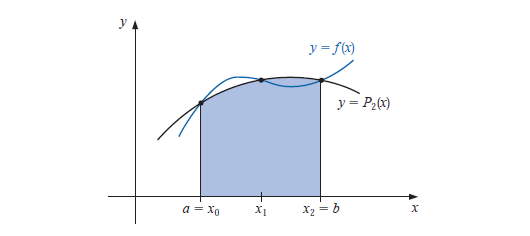
\includegraphics{images/simpsonapproximation}
\caption{Aproximação de \textit{y=f(x)} por \textit{y=$P_{2}$(x).}}
\end{figure}


\quad Para casos em que o intervalo [a,b] seja pequeno a ponto que a função \textit{f(x)} seja suave, a aproximação de Simpson calcula a integral exatada para esse intervalo. Incialmente o intervalo [a,b] pode não ser suficientemente pequeno para que a aprximação convirja para o valor exato. Nessas situações é possível quebrar o intervalo em subintervalos menores e aplicar a regra de Simpson para cada um desses subintervalos. A aproximação da integral de \textit{f(x)} nesse caso será dada pela soma da aproximação de cada intervalo. Para o caso em que divide-se o intervalo [a,b] em subintervalos para obter a aproximação mais exatada da função, a regra é chamda de Simpson Composta.\\

\newpage

\quad Em Simpson Composto divide-se o intervalo [a,b] em \textit{n} subintervalos, sendo \textit{n} um número par. Então, a aproximação da função \textit{f(x)} é dada por:

\begin{equation}
\int_{a}^{b} f(x)dx \approx \dfrac{(b-a)}{3n} [f(a) + \sum_{i=1}^{(n/2)-1}4f(x_{2j})+ \sum_{i=1}^{(n/2)-1}4f(x_{2j-1}) + f(b)] 
\end{equation}

\begin{figure}[h]
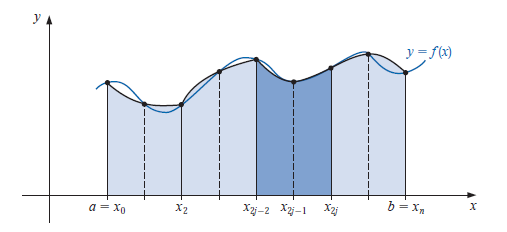
\includegraphics{images/simpsoncompositeapproximation}
\caption{Aproximação de \textit{y=f(x)} pela soma das integrais dos subintervalos [a,b].}
\end{figure}

\newpage
\subsection{Quadratura Gaussiana}

\qquad A Quadratura Gaussiana, assim como a regra de Simpson, é um método de aproximação numérico para integrais definidas. Contudo, para uma aproximação utilizando \textit{n} pontos de integração, o valor da integral será exato para polinômios de até $2\textit{n}-1$ ordem. O método da Quadratura Gausiana propõe abscissas ótimas para o cálculo afim de minimizar o erro, como representado na Figura 3 por $x_{1}$ e $x_{1}$, ao invés de usar os pontos das extremidades do intervalo [a,b]. Ainda, são levados em considerações os fatores denominados pesos $w_{i}$. 

\begin{figure}[h]
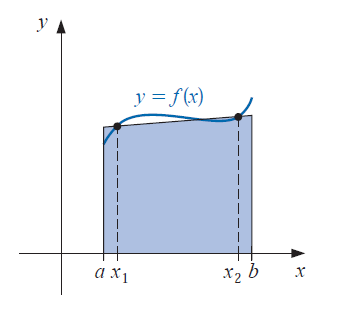
\includegraphics{images/gaussapproximation}
\caption{Escolha de abscissas ótimas para a integração de \textit{f(x)}}
\end{figure}

\qquad É possível utilizar os polinômios de Legendre para determinar os pontos das abscissas $x_{i}$ para o intervalo [-1,1], dados como as raízes do polinômio de Legendre (\textit{$P_{n}$}) para ordem \textit{n}. E os pesos $w_{i}$ são dados por:

\begin{equation}
w_{i}=\dfrac{2}{(1-x^2_{i})[P'_{n}(x_{i})]^2}
\end{equation}

\qquad Então, com os pesos e abscissas determinados para \textit{n} pontos de integração, a aproximação é dada por:

\begin{equation}
\int_{-1}^{1} f(x)dx \approx \sum_{i=1}^{n} w_{i}f(x_{i})
\end{equation}

\qquad Dessa forma obtém-se o valor da integração para os limites [-1,1], porém os limes de integração podem ser difentes desse, para isso, coverte-se os limites de integração para qualquer intervalo [a,b] por: 

\begin{equation}
\int_{a}^{b}f(x)dx=\dfrac{b-a}{2}\int_{-1}^{1}f(\dfrac{b-a}{2}x_{i}+\dfrac{b+a}{2})\approx\dfrac{b-a}{2}\sum_{i=1}^{n}w_{i}f(\dfrac{b-a}{2}x_{i}+\dfrac{b+a}{2})
\end{equation}


\newpage
\subsection{Programação}
\qquad Foi utilizado o programa Wolfram Mathematica para analisar o desempenho dos métodos de Simpson e a Quadratura Gaussiana. Assim, foram escritos dois métodos de resolução, um para cada aproximação. Para ambos os métodos foram definidos a mesma função \textit{f(x)}, o memos intervalo de integração [a,b] e um fator \textit{p}. Para a Quadratura de Gauss o valor de \textit{p} será o número de pontos de integração e para a Regra de Simpson, ese valor será a metade do número de sub intervalos criados. Ainda, foi adotada a precisão de $10^{-10}$ como sendo um valor aceitavelmente próximo ao valor da integral, ou seja, quando o valor aproximado pelos métodos tiver uma diferença menor que $10^{-10}$ com relação ao valor real da integral, é cosiderado que o método convergiu exatamente.\\

\quad Abaixo seguem três exemplos do funcionamento dos métodos, mostrando a relação entre os erros gerados para cada número de pontos/subintervalos:\\

\quad Para a função $f(x)=cos(2x^2)$, no intervalo de [0,1] com $p=10$ (20 subintervalos para a Regra de Gauss e 10 pontos para a Quadratura de Gauss), temos:

\begin{figure}[h]
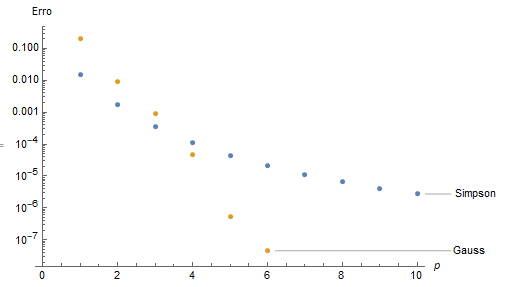
\includegraphics{images/erro_fcos}
\caption{Comparação de erros para $f(x)=cos(2x^2)$}
\end{figure}

\qquad O tempo que o Mathematica demorou para calcular os erros para a Regra de Simpson foi de 0.00217304 segundos, enquanto pela Quadratura Gaussiana o programa levou 0.00494727 segundos.

% Com os erros sendo: {0.209986, 0.00909262, 0.000927649, 0.0000469311, 5.39027*10^-7
% 4.56619*10^-8, 0, 0, 0, 0}

\newpage
\qquad Para os mesmos parâmetros escolhidos anteriormente, mas para a função $f(x)=e^{x^{2}}$ temos:

% Com os erros sendo: {0.178626, 0.00848386, 0.000242034, 4.93025*10^-6, 7.78885*10^-8, 
%1.00298*10^-9, 0, 0, 0, 0}

\begin{figure}[h]
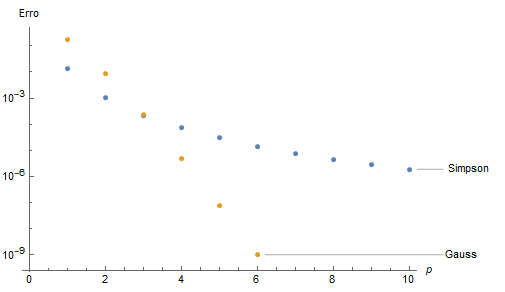
\includegraphics{images/erro_e}
\caption{Comparação de erros para $f(x)=e^{x^{2}}$}
\end{figure}

\qquad O tempo que o Mathematica demorou para calcular os erros para a Regra de Simpson foi de 0.0187616 segundos, enquanto pela Quadratura Gaussiana o programa levou 0.00394068 segundos.

\newpage
\qquad Para os mesmos parâmetros escolhidos anteriormente, mas para a função $f(x)=x^{21} + 3 x^7 + 45 x^2$ temos:

\begin{figure}[h]
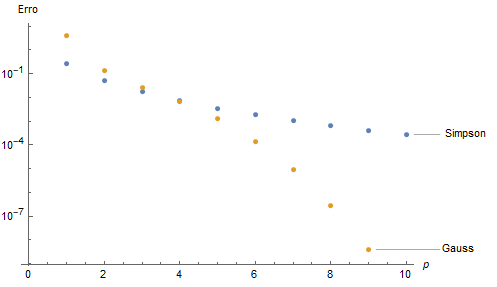
\includegraphics{images/erro_poli}
\caption{Comparação de erros para $f(x)=x^{21}+3x^7+45x^2$}
\end{figure}

\qquad O tempo que o Mathematica demorou para calcular os erros para a Regra de Simpson foi de 0.00387437 segundos, enquanto pela Quadratura Gaussiana o programa levou 0.00406029 segundos.\\

\newpage
\qquad Para esse exemplo foi aumentado o valor de \textit{p} da Regra de Simpson afim de que ela convergisse e foi notado que para $p=416$ o valor converge, conforme mostrado abaixo. Isso mostra que para 932 subintervalos do método de Simpson o método converge para um valor com $10^{-10}$ de diferença do valor da integral exata, enquanto o método da Quadratura de Gauss converge para essa mesma difrença com 10 pontos de integração. Ainda, o método de Simpsons demorou 3.78777 segundos para convergir para o resultado, enquanto o método de Gauss levou 0.00406029 segundos.

\begin{figure}[h]
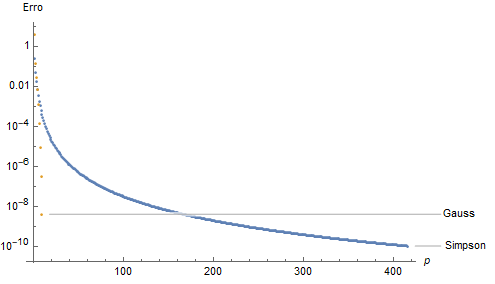
\includegraphics{images/erro_poli_convergindo}
\caption{Comparação de erros para $f(x)=x^{21}+3x^7+45x^2$ para ambos os métodos convergindo}
\end{figure}


\newpage
\section{Análise dos Resultados}
\qquad Visto os exemplos mostrados no item de Metodologia e Resultados percebe-se que a Quadratura de Gauss tem maior eficiência quando comparado a Regra de Simpsons, o que implica que o primeiro método converge para o resutado da integral de uma função com menos pontos de integração. Ainda, é importante levar em consideração que a curva de erros da Regra de Simpson tende a convergir para o valor exato com um valor grande de subintervalos. Conforme mostrado na Figura 7, foi visto que a curva de Simpson converge com $p=416$ enquanto Gauss converge com $p=10$, além de termos uma diferença de tempo de execução do programa de aproximadamente 3.7878 segundos para o método de Simpson contra 0.0041 segundos para o método de Gauss.\\

\qquad Imaginando um cenário em que o intervalo [0,1] estudado seja apenas um pequeno intervalo dentro de um intervalo [a,b], onde um possível estudo se baseie, podem ser necessárias milhares de integrações em pequenos intervalos. Isso implica que para integrar um intervalo [a,b], tavez seja necessário milhares de vezes o tempo necessário para integrar um intervalo pequeno, como o [0,1]. Assim percebe-se que o método de Gauss torna-se mais interessante quando comparado a Rega de Simpson.
\newpage

\end{document}
